% Feature engineering and K-Means location clustering
\begin{frame}{Feature Engineering: 30 Features}
  \begin{columns}[T]
    \begin{column}{0.51\textwidth}
      \small
      \begin{tabular}{p{1.5cm}p{4.9cm}}
        \toprule
        Group & Features \\
        \midrule
        Spatial &
          latitude, longitude, corridor, police station, zone, junction,
          \textbf{location cluster} \\
        Temporal &
          hour, minute, day of week, month, day, weekend flag,
          morning- and evening-rush flags, time-of-day bucket \\
        Contextual &
          event type, event cause, vehicle type, duration, status,
          weather flag \\
        \bottomrule
      \end{tabular}

      \vspace{3mm}
      \begin{block}{Encoding and splitting}
        \small Nine categorical columns label-encoded, numerics standardised.
        Both transformers are \textbf{serialized}, so a new event is encoded exactly
        as in training. Split 6{,}538 / 1{,}635, \textbf{stratified}.
      \end{block}
    \end{column}
    \begin{column}{0.47\textwidth}
      \centering
      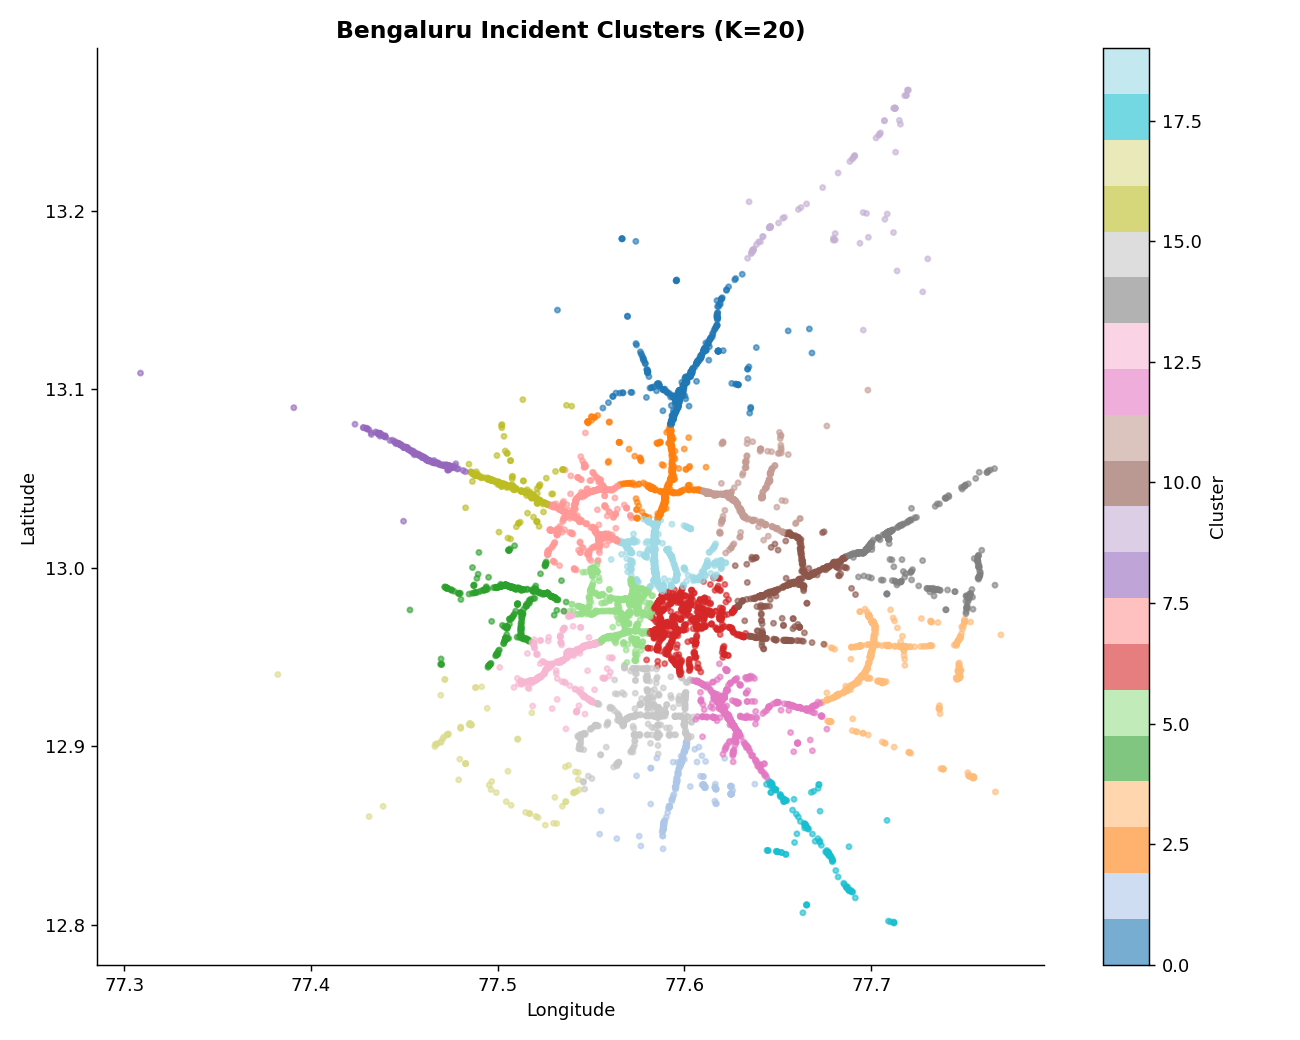
\includegraphics[width=\textwidth]{figs/geo_clusters.png}

      \vspace{1mm}
      {\scriptsize \textbf{K-Means, $K = 20$}: unsupervised grouping of the
      8{,}173 event coordinates; the cluster ID becomes feature 30.}
    \end{column}
  \end{columns}
\end{frame}
